\chapter{Preliminary Wing Box Design}
\label{ch:Prelim_WB_Des}
\noindent The wing box is the primary wing structure which serves as the base for all wing components. It needs to be designed in such a way that the whole wing will be able to cope/withstand all forces (bending, torsion, shear, etc.) acting on it during all parts of a flight. Firstly, the overview of the design procedure is presented in \autoref{sec:design procedure}. Secondly, the specific functions of the wing box will be stated in \autoref{sec:FuncAnalWinbox}. These functions were found based on calculations performed earlier in \autoref{ch:ForceDiagram} and 
\autoref{ch:Stiff_Calc}. In \autoref{sec:Loading_Diagrams} six different V-n diagrams were derived from the specified conditions. Next in \autoref{sec:Tab_LoadCase} load cases are defined based on $\left(V_{EAS}-n\right)$ diagrams. These load cases are later used in \autoref{sec:Prelim_Des_Ops} to came up with three design options that meet the critical requirements stated earlier in \autoref{sec:Req_Anal_WB}.

\begin{comment}
    
One of these functions is being able to withstand the loads and moments determined in \autoref{ch:ForceDiagram}, while adhering to the critical requirements set in \autoref{ch:Stiff_Calc}. Those loads were found using the $\left(V_{EAS}-n\right)$ diagrams in \autoref{sec:Loading_Diagrams}. The diagrams then created the so-called load cases, where the loads on the wing box would be the highest. These specific scenarios are highlighted in \autoref{sec:Tab_LoadCase}. The requirements set in \autoref{ch:Stiff_Calc} will then in combination with the scenarios from \autoref{sec:Tab_LoadCase}, generate the final wing box requirements in \autoref{sec:Req_Anal_WB}. \autoref{sec:Prelim_Des_Ops} will then fulfill these requirements by generating three separate wing box designs.
\end{comment}

\section{Wing box design procedure}
\label{sec:design procedure}
Wing box design is a complicated and iterative process that requires the usage of tools obtained earlier in \autoref{ch:ForceDiagram} and \autoref{ch:Stiff_Calc}. The first part of the design process is to obtain a manoeuvre-loading diagram for several flight cases to use them to define appropriate loading cases. These load cases along with force diagrams obtained earlier in \autoref{ch:ForceDiagram} were used to define final critical requirements that directly influenced the design. At this point, all three designs could have been proposed. The design team came up with three designs (based on different philosophies) that were later checked with the tool obtained in \autoref{ch:Stiff_Calc} to meet the critical requirements. Finally, the process of checking the requirements along with optimizing the preliminary design was performed several times to get three designs that meet all critical requirements stated earlier. The overview of the whole procedure is presented on the \autoref{fig:flowchart}.




\usetikzlibrary{shapes.geometric, arrows}



\definecolor{70af333d-4869-5f2a-97ca-9904a9fce6c3}{RGB}{179, 254, 174}
\definecolor{f3551e38-74df-57e2-b793-83d7fe876c85}{RGB}{0, 0, 0}
\definecolor{0b71a967-1f15-55a5-9bb9-70efa7b4fc58}{RGB}{51, 51, 51}
\definecolor{747aec21-333b-59ee-84e3-ddff893e5ccd}{RGB}{255, 216, 176}
\definecolor{adaee4ed-88c8-5b21-a9e7-31316ebef86f}{RGB}{255, 179, 178}
\definecolor{5856d031-3da1-575c-834e-c77e9e438c62}{RGB}{162, 177, 195}

\tikzstyle{WP2-diamond} = [diamond, minimum width=3cm, minimum height=2cm, text centered, font=\large, color=0b71a967-1f15-55a5-9bb9-70efa7b4fc58, draw=f3551e38-74df-57e2-b793-83d7fe876c85, line width=1, fill=70af333d-4869-5f2a-97ca-9904a9fce6c3]
\tikzstyle{V-n-Rectangle} = [rectangle, minimum width=3cm, minimum height=1cm, text centered, font=\normalsize, color=0b71a967-1f15-55a5-9bb9-70efa7b4fc58, draw=f3551e38-74df-57e2-b793-83d7fe876c85, line width=1, fill=747aec21-333b-59ee-84e3-ddff893e5ccd]
\tikzstyle{c1348099-d7cb-5a2d-89c5-daa2787c1591} = [rectangle, minimum width=3cm, minimum height=1cm, text centered, font=\normalsize, color=0b71a967-1f15-55a5-9bb9-70efa7b4fc58, draw=f3551e38-74df-57e2-b793-83d7fe876c85, line width=1, fill=747aec21-333b-59ee-84e3-ddff893e5ccd]
\tikzstyle{512bdd77-c3aa-5669-a956-85f7a90c6fb4} = [rectangle, rounded corners, minimum width=3cm, minimum height=1cm, text centered, font=\normalsize, color=0b71a967-1f15-55a5-9bb9-70efa7b4fc58, draw=f3551e38-74df-57e2-b793-83d7fe876c85, line width=1, fill=adaee4ed-88c8-5b21-a9e7-31316ebef86f]
\tikzstyle{7be24b85-97d0-5b76-ba9e-d94005dca8f2} = [thick, draw=5856d031-3da1-575c-834e-c77e9e438c62, line width=2, ->, >=stealth]


\begin{figure}[H]
    \centering
\begin{tikzpicture}[node distance=2cm]

\node (5ad49ccc-6515-4d1c-b24b-cd30eb88c845) [V-n-Rectangle, below of=9214c975-5b8d-40a1-a919-5f0ca9435a02, yshift=-0.5cm] {n-V Diagrams};
\node (9214c975-5b8d-40a1-a919-5f0ca9435a02) [WP2-diamond, above of=5ad49ccc-6515-4d1c-b24b-cd30eb88c845, xshift=4cm] {WP 4.1};
\node (d15626ae-577c-46b5-ab8e-b609b527d898) [WP2-diamond, right of=9214c975-5b8d-40a1-a919-5f0ca9435a02, xshift=2cm] {WP 4.2};

\node (77d529d5-6f80-4ba7-852d-5db0a8bfabfe) [V-n-Rectangle, right of=5ad49ccc-6515-4d1c-b24b-cd30eb88c845, xshift=2cm] {Load Cases};
\node (2781bf06-b5d3-47c0-a90f-68879a683784) [c1348099-d7cb-5a2d-89c5-daa2787c1591, right of=5ad49ccc-6515-4d1c-b24b-cd30eb88c845, xshift=6cm] {Critical Requirements};
\node (9b8095fe-e9a2-4d7b-95f7-1b296a4bc41f) [512bdd77-c3aa-5669-a956-85f7a90c6fb4, right of=5ad49ccc-6515-4d1c-b24b-cd30eb88c845, xshift=10cm] {Three Designs};
\node (46582238-2501-40fd-9703-900311286e92) [V-n-Rectangle, below of=5ad49ccc-6515-4d1c-b24b-cd30eb88c845, xshift=10cm] {CHECK!};
\draw [7be24b85-97d0-5b76-ba9e-d94005dca8f2] (77d529d5-6f80-4ba7-852d-5db0a8bfabfe) --  (2781bf06-b5d3-47c0-a90f-68879a683784);
\draw [7be24b85-97d0-5b76-ba9e-d94005dca8f2] (5ad49ccc-6515-4d1c-b24b-cd30eb88c845) --  (77d529d5-6f80-4ba7-852d-5db0a8bfabfe);
\draw [7be24b85-97d0-5b76-ba9e-d94005dca8f2] (2781bf06-b5d3-47c0-a90f-68879a683784) --  (9b8095fe-e9a2-4d7b-95f7-1b296a4bc41f);
\draw [7be24b85-97d0-5b76-ba9e-d94005dca8f2] (9214c975-5b8d-40a1-a919-5f0ca9435a02) --  (77d529d5-6f80-4ba7-852d-5db0a8bfabfe);
\draw [7be24b85-97d0-5b76-ba9e-d94005dca8f2] (d15626ae-577c-46b5-ab8e-b609b527d898) --  (2781bf06-b5d3-47c0-a90f-68879a683784);
\draw [7be24b85-97d0-5b76-ba9e-d94005dca8f2] (9b8095fe-e9a2-4d7b-95f7-1b296a4bc41f) |-  (46582238-2501-40fd-9703-900311286e92);
\draw [7be24b85-97d0-5b76-ba9e-d94005dca8f2] (46582238-2501-40fd-9703-900311286e92) -|  (2781bf06-b5d3-47c0-a90f-68879a683784);
\end{tikzpicture}
    \caption{Wing box design procedure visualisation}
    \label{fig:flowchart}
\end{figure}


\section{Wing Box Functional Analysis}
\label{sec:FuncAnalWinbox}
\autoref{tab:Wingbox_functions} presents the main functionalities that a wing box should provide. All of them were taken into account during the iterative design process.

\begin{table}[H]
    \centering
    \caption{Functions of a Wing box}
    \begin{tabularx}{\textwidth}{|p{.2\textwidth} |p{.745\textwidth}|}
        \hline
        \cellcolor{blue!15}\textbf{Code} & \cellcolor{blue!15}\textbf{Function} \\
        \hline

        \cellcolor{blue!15} FUN-BOX-01 & \textit{Provide a load-bearing structure to the wing.}\\
        \hline
        \cellcolor{blue!15} FUN-BOX-02 & \textit{Provide structural rigidity to the wing.}\\
        \hline
        \cellcolor{blue!15} FUN-BOX-03 & \textit{House the fuel stored in the wing.}\\
        \hline
        \cellcolor{blue!15} FUN-BOX-04 & \textit{Provide a way to attach the Control Surfaces to the wing.}\\
        \hline
        \cellcolor{blue!15} FUN-BOX-05 & \textit{Provide housing and protection for the electronics in the wing.}\\
        \hline
        \cellcolor{blue!15} FUN-BOX-06 & \textit{Provide extra resistance to flutter.}\\
        \hline
        \cellcolor{blue!15} FUN-BOX-07 & \textit{TBD}\\
        \hline
        \cellcolor{blue!15} FUN-BOX-08 & \textit{TBD}\\
        \hline
        
        
    \end{tabularx}
      
        \label{tab:Wingbox_functions}
\end{table}

\section{Manoeuvre Loading Diagram}
\label{sec:Loading_Diagrams}

\noindent Finding the load cases requires drawing the manoeuvre loading diagram, also called V-n diagram, for different altitudes and weights considered. This graph shows which load factors correspond to the aircraft's most characteristic speeds. Here six different V-n diagrams will be provided by analysing the aircraft flying at cruise and sea altitude at the following three weight configurations: OEW, OEW + MPW, and OEW + MPW + MF such that MTOW is obtained. \autoref{fig:v-ncaseCrit} shows the most critical V-n diagram which corresponded to... \autoref{v-n_diagrams} contains the other five V-n diagrams. In order to draw these diagrams the following characteristic velocities and loading factors were used:

\begin{itemize}
    \item $V_{S0}$: stall speed with flaps extended. \autoref{eq:v_so}, taken from \textit{"AE2111-I: System Design - Project Reader" } \cite{Timmer2024AE2111-IReader}, was used. Here $W$ was replaced for each one of the weights in the three cases, $\rho$ corresponds to the sea level or cruise density, depending on the case being analysed, $C_{L_{max _{land}}}$ has a value of $2.5$, and the surface area of the wing (denoted by $S$) is $265.21$ m$^2$. %add reference to our previous report (report III)
    \begin{equation}
    \label{eq:v_so}
        V_{S0} = \sqrt{\frac{2W}{C_{L_{max _{land}}} \rho S}} 
    \end{equation}
    \item $V_{S1}$: stall speed with flaps retracted. \autoref{V_s1} \cite{Timmer2024AE2111-IReader} was used in this case. Variables in this equation are the same as the ones mentioned for $V_{S0}$, the only changing parameter is $C_{L_{max _{clean}}}$, which takes a value of $1.7$.
    \begin{equation}
    \label{V_s1}
         V_{S1} = \sqrt{\frac{2W}{C_{L_{max _{clean}}} \rho S}}
    \end{equation}
    \item $V_A$: manoeuvring speed. This was calculated by using \autoref{v_a} \cite{Timmer2024AE2111-IReader}. The variables in this equation are again the same as the ones used for $V_{S0}$. The new variable is $n_{max}$ which corresponds to a value of $2.5$ in the cases being analysed. 
    \begin{equation}
    \label{v_a}
        V_A = \sqrt{\frac{2n_{max}W}{C_{L_{max_{clean}}}S\rho}}
    \end{equation}
    \item $V_C$: cruise speed. This was given to be 241.96 ms$^{-1}$ \cite{Timmer2024AE2111-IReader}.
    \item $V_D$: design dive speed. The calculation for this speed is can be directly calculated by using \autoref{v_d} \cite{Timmer2024AE2111-IReader}.
    \begin{equation}
    \label{v_d}
        V_D = 1.5V_C
    \end{equation}
    
    \item $V_F$: design wing-flap speed. This parameter was calculated by choosing the highest velocity out of: $1.6V_{s1}$, $1.8V_{s1}$, $1.8V_{s0}$ and $V_{intersect}$, which was calculated by multiplying $V_{s1}$ by $\sqrt{2}$.
    
    \item $n_{max}$: positive limit manoeuvring load factor. This value may not be less than $2.5$ or higher than $3.8$. It can be calculated by using \autoref{n_max} \cite{Timmer2024AE2111-IReader}. For all of the considered cases, $n_{max}$ was lower than $2.5$, therefore $n_{max}$ resulted in a value of $2.5$ for all cases. 
    \begin{equation}
    \label{n_max}
        n_{max} = 2.1 + \frac{24000}{W+10000}
    \end{equation}
    
    \item $n_{min}$: negative limit for manoeuvring load factor. This value could not be less than $-1$. Therefore this was the assumed value for all cases \cite{Timmer2024AE2111-IReader}.
    \item The maximum load factor with flaps deflected was assumed to be $2.0$, according to \textit{"AE2111-I: System Design - Project Reader" } \cite{Timmer2024AE2111-IReader}.
\end{itemize}

\begin{figure}[H]
    \centering
    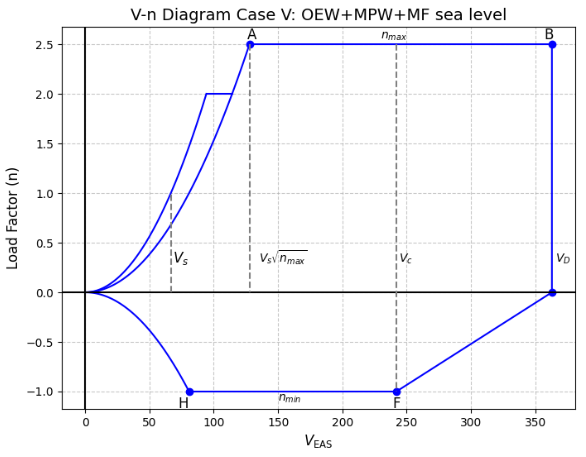
\includegraphics[width=0.65\linewidth]{figures/v-n diagram case V.png}
    \caption{V-n diagram for the aircraft operating at OEW, MPW and MF; at sea level conditions} 
    \label{fig:v-ncaseCrit}
\end{figure}

\section{Table of Load Cases}
\label{sec:Tab_LoadCase}
As six different manoeuvre loading diagrams were obtained in the previous section (\autoref{sec:Loading_Diagrams}), they can be used to develop appropriate load cases that will later be used to define critical design requirements. By looking at \autoref{fig:v-ncaseCrit} five critical load cases can be found for each one of the V-n diagrams:
%add reference to any V-n diagram
\begin{itemize}
    \item Point A: This point represents the maximum load factor $n_{max}$ the aircraft can experience at the manoeuvring speed ($V_A$). If the load factor is further increased the aircraft will experience structural damage.
    \item Point B: This is the maximum positive load factor at the design dive speed $V_D$, for safety reasons, the aircraft cannot overpass this limit. 
    \item Point F: Corresponds to the minimum load factor the aircraft can handle at cruise speed ($V_c$). 
    \item Point H: This load case corresponds to the minimum load factor the aircraft can experience, corresponding to $V_{s1}$.
    \item Horizontal intersection at n = $2$: Maximum load factor the aircraft can handle with flaps down.
\end{itemize}

\noindent These load cases are then shown for each combination of Weight and Altitude considered. The results obtained are shown in \autoref{tab:LoadCases}.



\begin{longtable}{|>{\columncolor{blue!15}}c|p{3.2cm}|p{2cm}|c|c|c|p{2.6cm}|}
\caption{Table of considered Load Cases}
\label{tab:LoadCases}
\endfirsthead
    \hline
    \rowcolor{blue!15} \textbf{Load Case} & \textbf{Description} & \textbf{Speed$_{EAS}$ [m s$^-1$]} & \textbf{Altitude} & \textbf{Weight [N]} & \textbf{n} & \textbf{Comments} \\
    \hline
    LC-1 & OEW Sea Level at $V_{d}$ & 362.94 & FL0 & 770060.92 & 2.5 & Trimmed HLDs (clean config.) \\
    \hline
    LC-2 & OEW Sea Level at $V_{c}$ & 241.96 & FL0 & 770060.92 & -1 & Trimmed HLDs (clean config.) \\ 
    \hline
    LC-3 & OEW Sea Level at $V_{f,intersection}$ & 74.68 & FL0 & 770060.9165 & 2 & This is with full flaps \\ \hline
    LC-4 & OEW Sea Level at $V_{a}$ & 83.50 & FL0 & 770060.92 & 2.5 & Trimmed HLDs (clean config.) \\ 
    \hline
    LC-5 & OEW Sea Level at $V_{S1}$ & 52.81 & FL0 & 770060.92 & -1 & Trimmed HLDs (clean config.) \\ 
    \hline
    LC-6 & OEW Cruise Level at $V_{d}$ & 184.47 & FL390 & 770060.92 & 2.5 & Trimmed HLDs (clean config.) \\ 
    \hline
    LC-7 & OEW Cruise Level at $V_{c}$ & 122.98 & FL390 & 770060.92 & -1 & Trimmed HLDs (clean config.) \\ 
    \hline
    LC-8 & OEW Cruise Level at $V_{f,intersection}$ & 74.68 & FL390 & 770060.92 & 2 & This is with full flaps \\ 
    \hline
    LC-9 & OEW Cruise Level at $V_{a}$ & 83.50 & FL390 & 770060.92 & 2.5 & Trimmed HLDs (clean config.) \\ 
    \hline
    LC-10 & OEW Cruise Level at $V_{S1}$ & 52.81 & FL390 & 770060.92 & -1 & Trimmed HLDs (clean config.) \\ 
    \hline
    LC-11 & OEW+MPW Sea Level at $V_{d}$ & 362.94 & FL0 & 1040574.12 & 2.5 & Trimmed HLDs (clean config.) \\ 
    \hline
    LC-12 & OEW+MPW Sea Level at $V_{c}$ & 241.96 & FL0 & 1040574.12& -1 & Trimmed HLDs (clean config.) \\ 
    \hline
    LC-13 & OEW+MPW Sea Level at $V_{f,intersection}$ & 86.81 & FL0 & 1040574.12 & 2 & This is with full flaps \\ 
    \hline
    LC-14 & OEW+MPW Sea Level at $V_{a}$ & 97.06 & FL0 & 1040574.12 & 2.5 & Trimmed HLDs (clean config.) \\
    \hline
    LC-15 & OEW+MPW Sea Level at $V_{S1}$ & 61.39 & FL0 & 1040574.12& -1 & Trimmed HLDs (clean config.) \\ 
    \hline
    LC-16 & OEW+MPW Cruise at $V_{d}$ & 184.47 & FL390 & 1040574.12 & 2.5 & Trimmed HLDs (clean config.) \\ 
    \hline
    LC-17 & OEW+MPW Cruise at $V_{c}$ & 122.98 & FL390 & 1040574.12 & -1 & Trimmed HLDs (clean config.) \\ 
    \hline
    LC-18 & OEW+MPW Cruise at $V_{f,intersection}$ & 86.81 & FL390 & 1040574.12 & 2 & This is with full flaps \\ 
    \hline
    LC-19 & OEW+MPW Cruise at $V_{a}$ & 97.06 & FL390 & 1040574.12 & 2.5 & Trimmed HLDs (clean config.) \\ 
    \hline
    LC-20 & OEW+MPW Cruise at $V_{S1}$ & 61.39 & FL390 & 1040574.12 & -1 & Trimmed HLDs (clean config.) \\ 
    \hline
    LC-21 & OEW+MPW+fuel Sea Level at $V_{d}$ & 362.94 & FL0 & 1803421.35 & 2.5 & Trimmed HLDs (clean config.) \\ 
    \hline
    LC-22 & OEW+MPW+fuel Sea Level at $V_{c}$ & 241.96 & FL0 & 1803421.35 & -1 & Trimmed HLDs (clean config.) \\ 
    \hline
    LC-23 & OEW+MPW+fuel Sea Level at $V_{f,intersection}$ & 114.29 & FL0 & 1803421.35 & 2 & This is with full flaps \\ 
    \hline
    LC-24 & OEW+MPW+fuel Sea Level at $V_{a}$ & 127.78 & FL0 & 1803421.35 & 2.5 & Trimmed HLDs (clean config.) \\ 
    \hline
    LC-25 & OEW+MPW+fuel Sea Level at $V_{S1}$ & 80.81 & FL0 & 1803421.35 & -1 & Trimmed HLDs (clean config.) \\ 
    \hline
    LC-26 & OEW+MPW+fuel Cruise at $V_{d}$ & 184.47 & FL390 & 1803421.35 & 2.5 & Trimmed HLDs (clean config.) \\ 
    \hline
    LC-27 & OEW+MPW+fuel Cruise at $V_{c}$ & 122.98 & FL390 & 1803421.35 & -1 & Trimmed HLDs (clean config.) \\ 
    \hline
    LC-28 & OEW+MPW+fuel Cruise at $V_{f,intersection}$ & 114.29 & FL390 & 1803421.35 & 2 & This is with full flaps \\ 
    \hline
    LC-29 & OEW+MPW+fuel Cruise at $V_{a}$ & 127.78 & FL390 & 1803421.35 & 2.5 & Trimmed HLDs (clean config.) \\ 
    \hline
    LC-30 & OEW+MPW+fuel Cruise at $V_{S1}$ & 80.81 & FL390 & 1803421.35 & -1 & Trimmed HLDs (clean config.) \\ 
    \hline
\end{longtable}



\section{Requirement Analysis}
\label{sec:Req_Anal_WB}
Out of 30 Load Cases presented in \autoref{tab:LoadCases} only a few of them will define critical load requirements that the design will be based on. These load cases could be obtained using both qualitative and numerical reasoning.
\newline
The qualitative approach is based on assuming that for the highest airplane weight (OEW + MPW + fuel) the highest lift is needed thus that loading case will be critical. Load cases from 21 - 30 all assume the highest airplane weight but on different flight levels. Out of these ten load cases, we select those with both the highest (2.5) and lowest (-1) load factors while ignoring cases with extended HLD (according to project reader \cite{Timmer2024ProjectDesign}). This procedure led to the selection of four critical loading cases (LC-21, LC-22, LC-26, LC-27) which were used to define critical requirements presented in \autoref{tab:req_list_wingbox}.
\newline
The numerical method was earlier described in \autoref{ch:ForceDiagram} and it will serve as confirmation of the after-mentioned qualitative approach.

\begin{comment}
    
After having obtained the most critical load cases in \autoref{sec:fd_critical_cases}, it is now possible to derive from them a requirements list for the wing box of the aircraft. This list is shown in \autoref{tab:req_list_wingbox}.
\end{comment}

\begin{longtable}[H]{|>{\columncolor{blue!15}}p{.2\textwidth} |p{.75\textwidth}|}
    \caption{Requirements list for the Wing box}
    \label{tab:req_list_wingbox}
    \endfirsthead
        \hline
        \textbf{Code} & \cellcolor{blue!15}\textbf{Function} \\
        \hline

         REQ-BOX-01-a & \textit{The wing tip shall not displace more than 15 \% of the wingspan when subjected to a load factor of $2.5$, whilst flying at an equivalent airspeed of $362.94$ ms $^{-1}$ at FL0, with maximum payload and no fuel, with all control surfaces retracted}\\
        \hline
         REQ-BOX-01-b & \textit{The wing tip shall not rotate more than $\pm 10 \degree $ of the wingspan when subjected to a load factor of $2.5$, whilst flying at an equivalent airspeed of $362.94$ ms $^{-1}$ at FL0, with maximum payload and no fuel, with all control surfaces retracted}\\
        \hline
        REQ-BOX-02-a & \textit{The wing tip shall not displace more than 15 \% of the wingspan when subjected to a load factor of $-1$, whilst flying at an equivalent airspeed of $241.96$ ms$^{-1}$ at FL0, with maximum payload and no fuel, with all control surfaces retracted}\\
        \hline
        REQ-BOX-02-b & \textit{The wing tip shall not rotate more than $\pm 10 \degree $ of the wingspan when subjected to a load factor of $2.5$, whilst flying at an equivalent airspeed of $241.96$ ms$^{-1}$ at FL0, with maximum payload and no fuel, with all control surfaces retracted}\\
        \hline
        REQ-BOX-03-a & \textit{The wing tip shall not deflect more than 15 \% of the wingspan when subjected to a load factor of $2.5$, whilst flying at an equivalent airspeed of $184.47$ ms$^{-1}$ at FL390, with maximum payload and no fuel, with all control surfaces retracted}\\
        \hline
        REQ-BOX-03-b & \textit{The wing tip shall not rotate more than $\pm 10 \degree $, when subjected to a load factor of $2.5$, whilst flying at an equivalent airspeed of $184.47$ ms$^{-1}$ at FL390, with maximum payload and full fuel, with all control surfaces retracted}\\
        \hline
        REQ-BOX-04-a & \textit{The wing tip shall not deflect more than 15 \% of the wingspan when subjected to a load factor of $-1$, whilst flying at an equivalent airspeed of $122.98$ ms$^{-1}$ at FL390, with maximum payload and full fuel, with all control surfaces retracted}\\
        \hline
        REQ-BOX-04-b & \textit{The wing tip shall not rotate more than $\pm 10 \degree $, when subjected to a load factor of $-1$, whilst flying at an equivalent airspeed of $122.98$ ms$^{-1}$ at FL390, with maximum payload and full fuel, with all control surfaces retracted}\\
        \hline
\end{longtable}

\section{Preliminary Design Options}
\label{sec:Prelim_Des_Ops}
This section will focus on the preliminary design of the wing box. The wing box can be designed with the requirements determined in \autoref{sec:Req_Anal_WB}. These designs will be based on different design philosophies resulting in vastly different structures.

\subsection*{Design Philosophies}
There is a wide range of design options that need to be considered to finally select one and achieve the required stiffness for the wing box. Each one of these options will have a different impact on the geometry, price and performance of the wing box. \\

\noindent The use of strong spars that carry most of the bending loads will help simplify the complexity of the design. However in this case the material was set to be AL2024-T81, therefore spars cannot be strengthened by used a different material. If this restriction did not exist, it would be recommended to consider other options. Another way to counteract this constrain would be increasing the thickness of the skin. The bad part of this solution would be the increase in weight and price of the design, as more material is being used. \\

\noindent A second option to increase the stiffness of the wing box is to place a high number of closely-spaced stringers. With this design the load will be more evenly distributed, and therefore its stiffness will increase. The downside of this option is that it increases the complexity of the design, and therefore manufacturing will increase the cost. \\

\noindent Another option to meet the torsional stiffness requirement is the use of several closed cells within the wing box. This design rapidly increases the stiffness, however complexity and weight will also increase. Alternatively the use of truss-like structures shall also be considered. If the geometry is optimized, the structure will flexible and capable of sustaining high loads while maintaining a low weight. 

\subsection*{Preliminary Results}
